From the perspective of an analyst examining a network, a typical workflow
would begin with considering all activity from a broad overview, using any
number of visualizations. Once a network attack has been identified, it should
be easy for the analyst to ``zoom in'' to the data of interest, by applying
successive filters to the source, and changing the representation to suit the
particular attack. Finally, when the exceptional behaviour has been singled
out, the analyst may explore details of the intrusion on demand.

This workflow illustrates the visual design framework suggested by Ben
Shneiderman, University of Maryland, in 1996;

\begin{center}
    \textit{Overview first, zoom and filter, then details-on-demand.}
\end{center}

To assist with the process of singling out suspicious activity, certain
visualizations allow filtering by mouse interaction. Where appropriate, the
analyst may click or drag their mouse cursor over sections of the active
visualization to create a new filter, or switch to a different representation
of the selected data. Navigation between complementing visualizations in this
fashion is highly intuitive and allows the analyst to tweak the active filters
quickly and effectively.

The following is a graphical representation of the typical workflow expected of
an analyst studying a network using NetVis.

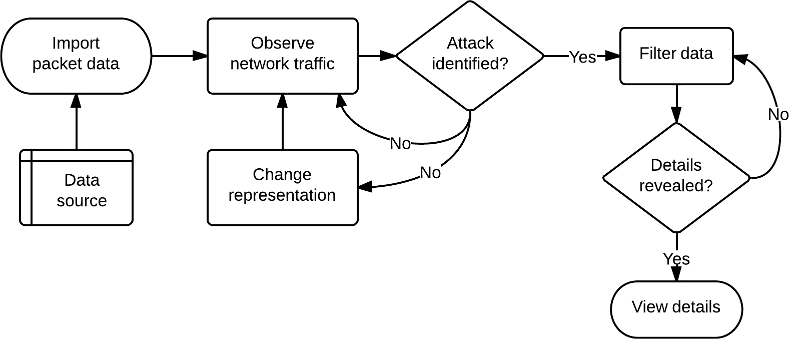
\includegraphics[width=\linewidth]{materials/workflow-diagram.png}
